% TODO expand, better intro
The Sybil attack clearly has a lot of consequences, some of them are very severe
and may cause financial lossess. In this section we categorise various defence
techniques against the sybil-attack. We classify them on their main idea, and
state explicitly when the mechanism is application specific.
% Many techniques are also hybrids, we explain these 

\subsection{Reputation Systems}
TODO PageRank\cite{baeza2005pagerank, cheng2006manipulability}

\subsection{Certificate Authority}\label{sec:cert-authority}
CA (certificate authorities) check the users' real identities and then issues
certificates to honest users. The certificate can be tangible (trusted
hardware~\cite{newsome2004sybil}) or non-tangible (public key certificate)
depending on the application. When an identity wishes to user the application,
the CA must verify the validity of its certificate to ensure one-to-one
correspondence. This mechanism prevents the Sybil attack as long as the CA does
not make mistakes in the issuance stage.

Many existing systems today use a form of CA. X.509~\cite{housley2002internet}
--- a standard for certificates, it is used in a large variety of applications.
For example, emails can be encrypted and signed using
S/MIME\cite{ramsdell2010secure} certificates which are based on X.509. Attackers
can still create a large number of Sybils and send emails, but the receiver
would reject the emails because they are not correctly signed.

CA can prevent the Sybil attack but it also has a lot of downsides. (1) Users
have different opinions and may not agree on a single CA. (2) Users living in
authoritarian regimes may not have access to the necessary CA. (3) It is
difficult to scale up a CA to meet increasing users demands. (4) Anonymity is
difficult to obtain because the CA has complete information of the entities. (5)
It is a central point of failure; i.e. if the attacker obtains the private key
to create certificates then he or she can easily generate Sybils, if the CA goes
offline then the application ceases to function because it can no longer verify
identites.

% Credence\cite{walsh2006experience} is a distributed reputation system, but the
% identities are created using a CA.

\subsection{Resource Testing}\label{sec:resource-testing}
Resource testing makes attacks costly. That is to say every attacker can create
multiple sybils, but the attack cannot duplicate its resources the same way. The
resource type varies depending on the application, and we give a few examples
below. It may deter casual attackers but its usefulness degrades for resourceful
attackers.

% In wireless networks it may be using radio
% channels\cite{newsome2004sybil}, in online social networks it may be IP
% addresses\cite{freedman2002tarzan} and solving computationally demanding puzzles
% in P2P networks\cite{aspnes2005exposing}.

In P2P networks, IP address can be used as a resource. In
Tarzan~\cite{freedman2002tarzan}, neighbours are selected not from all known IP
addresses, but from distinct IP prefixes. The effectiveness of the Sybil attack
is reduced if the attackers cannot easily create Sybils in a large range of IP
prefixes. Another example the self-registration
technique~\cite{dinger2006defending}. When a peer wish to join the network, it
needs to compute a ID which is a cryptographically secure hash of its own IP
address and port number, and then broadcast it to the network. While
participating in the nettwork, other peers need to verify that the ID matches
the peer's origin.

Aspnes et el. proposed the idea of solving difficult puzzles to limiting the
number of sybils~\cite{aspnes2005exposing}. The puzzle in this case is computing
hashes on some input $y$ concatinated by a some string $x$ such that the digest
begins with $w$ number of zeros. Essentially, every node acts as a verifier by
picking $y$ and then broadcast it to the network to the puzzle
solver\footnote{We simplify the protocol a bit because the original protocol
  (called Democracy) is made to be Byzantine fault tolerent and is a bit more
  involved.}. The puzzle solver must compute as many $x$ as possible such that
they match the requirement. Sybils are unlikely to produce enough $x$'s so the
honest nodes will refuse to interact with them.

In fact, many crypto-currencies use the same idea. For instance
\emph{proof-of-work} in Bitcoin~\cite{nakamoto2008bitcoin}. The Bitcoin
blockchain is a global ledger and it needs to reach a concensus for its blocks.
Nodes in the Bitcoin network essentially ``vote'' for the the latest block. But
the vote is performed not by counting the majority, but by ``counting'' the
amount of CPU power, i.e. one CPU is one vote. Thus an attacker cannot simply
create a lot of identities to out-vote the honest nodes. It needs to gather a
lot of CPU power which is much more difficult.

% SybilConf\cite{tegeler2010sybilconf}

\subsection{Registration Fee}\label{sec:registration-fee}

Friedman and Resnick is one of the first to propose the use of a registration
fee~\cite{resnick2001social}. It is similar to resource testing except it only
happens on registration. Entities can be charged a fee for creating identities,
often facilitated by a central authority. The fee needs to be set appropriately
so that the cost of creating Sybils outweights the benefits but does not hinder
honest entities.

The fee does not need to be monetary. For instance, Friedman and Resnick
proposed the idea of a once-in-a-lifetime identity\cite{resnick2001social}. It
uses blind signatures and a central authority, the authority does not know the
mapping between the real identity (e.g. driving licence) and the pseudo identity
of entities, but it checks whether there has been previous registrations of the
same real identity. In this case, the fee is the real identity, and attackers
cannot create an arbitrary number of real identities.
CAPTCHA~\cite{von2003captcha} is another form of registration fee. It prevents
programs from automatically creating new identities and limits the rate at which
identities can be created by asking users to solve a puzzle that is difficult
for computers.

Feldman et el. proposed another form of registration fee for P2P networks - the
adaptive stranger policy\cite{feldman2004robust}. When new peers join the
network, they are treated using a policy that is adapted from previous
newcomers. For example, the new peers may be expected to contribute to the
network before they are allowed to receive benefits from the ``mature'' peers.
The downside is that the policy may deter honest users from joining the network
in the first place.

% Identity creation can be rate limited\cite{douceur2002sybil}, especially in the
% presence of a central authority. The limit can be set globally, or it can be
% done regionally (i.e. based on IP address).

\subsection{Network Flow}\label{sec:network-flow}
Network flow based techniques began with
BarterCast\cite{meulpolder2009bartercast}. It was initially designed to combat
freeriding in P2P file sharing networks, where users are selfish and do not
share content, but its idea can be extended combat the Sybil attack. The ideas
based on BarterCast do not directly identify Sybils, but they prevent Sybils
from doing harm in the P2P network.

The main idea comes from human interactions, where the reputation of a person
can be from direct experiences, or information obtained frome someone else. The
direct experience is always true, but the indirect information may not be, i.e.
people can lie about their experiences. Humans solve the problem by treating the
indirect information with a grain of salt unless the source of the information
is highly trusted.

BarterCast applies this idea in P2P file sharing networks. Peers all maintain a
subjective graph which is created by exchanging messages with their neighbours.
The direct experiences measured by the number of bytes uploaded and downloaded
are represented by the outgoing and incoming edges from the peer, respectively.
Indirect experiences are represented by edges that are not directly connected to
the peer. For example in \autoref{fig:bartercast}, $A$ is the subject, it has
direct experiences with $B$ and $B$ has told $A$ about $S$, so it has indirect
information about $S$. But $A$ is unsure about the truthfulness of $S$'s
contribution, so it only trusts $S$ as much as it trusts $B$. This idea is
realised using the Ford-Fulkerson maximum flow
algorithm~\cite{thomas2001introduction} as shown in \autoref{fig:bartercast},
$A$ only have 5 units of trust for $S$ even when $S$ apparently contributed a
lot to $B$.

\begin{figure}
  \centering
  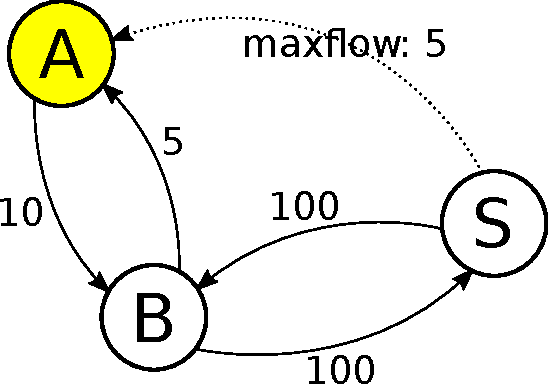
\includegraphics[width=0.3\textwidth]{bartercast}
  \caption{Subjective graph of $A$. The numbers are the amout of data transfered,
    they can be seen as the capacity in the context of the maximum flow
    problem.}
  \label{fig:bartercast}
\end{figure}

BarterCast does not prevent the Sybil attack by itself. Because attackers can
first upload a lot of data to obtain a good reputation in the network. If the
attacker now creates Sybils and false report of the Sybils saying that they
uploaded a lot. Then the peers who have interacted with the attacker will be
tricked to think that the Sybils also have a high reputation. To fix this
problem, Delaviz et el. created SybilRes~\cite{delaviz2012sybilres}.
% TODO draw?
The main idea is the following. Suppose there are two peers $A$ and $B$ who are
sharing data. If $A$ is uploading (represented by an outgoing edge) to $B$, then
it decreases the weight of the incoming edge from $B$. Vice versa, the weight is
increased for the outgoing edge when $A$ is downloading. The rate of change
depends on the capacities of the edges and the amout of data transferred after
computing the reputation. Using the definition in \autoref{fig:attack-edge}, the
attacker cannot built up reputation for its Sybils by uploading to peers in the
honest region beforehand, it is now forced to keep on uploading to keep its
Sybil's reputation which is a much more desirable behaviour.

Seuken et al. provided a formal model of BarterCast. They found that BarterCast
is vulnerable to misreporting and proposed a solution called the DropEdge
mechanism~\cite{seuken2011sybil, seuken2014sybil}. DropEdge, like the name
implies, drops some edges in the subjective graph that satisfies the following
constraints. Suppose peer $A$ wishes to download from peers in set $C$ (the
choice set). Then any reports received by $A$ from $p \in C$ is dropped. Also,
edges with both end points in $C$ are also dropped from $A$'s subjective graph.
Peers in $C$ cannot misreport their contribution since all the necessary edges
are dropped. The authors prove that it is robust against weakly beneficial
sybils, that is sybils that do not perform actual work for honest peers. The
authors also prove that no mechanism can prevently strongly beneficial sybils,
i.e. sybils that interact with honest users.

SumUp\cite{tran2009sybil} is a defence mechanism specific for the vote
aggregation problem. For example, in social news aggregation websites such as
Reddit\footnote{\texttt{www.reddit.com}}, users vote on the submitted content to
determine its ranking; the problem occurs when Sybils can out-vote honest users.
It is a centralised approach that fits the architecture of most websites that
perform vote aggregation. SumUp consist of three stages. Firstly, pruning is
performed to limit the number of incoming edges of every node, this is to reduce
the number of attack edges available and reduce the computational cost in later
stages, the threshold for the number of edges to prune is a system parameter.
Secondly, it uses a ticket source (the central component) to distribute tickets
in a breadth-first search manner equally to its neighbours, every node keeps one
ticket and distributes the remaining tickets the same way. The number of tickets
distributed across an edge plus one is the capacity of the edge. Effectively,
edges closer to the ticket source have a high capacity. This idea keeps the
capacities in the Sybil region low so that they do not have a large influence on
the outcome. Finally, the maximum flow is computed where the source is simply
the ticket source and the sink is an imaginary node with edges of capacity one
that is connected to every voter. SumUp offers a better guarantee than
SybilLimit (\autoref{sec:random-walk}) where it only accepts $1 + o(n)$ votes
per attack edge. Unlike the aforementioned techniques in this section,
SumUp requires a social network so it does not work in a generic P2P setting. An
improved version of SumUp - GateKeeper is discussed in
\autoref{sec:random-walk}.

\begin{figure}
  \centering
  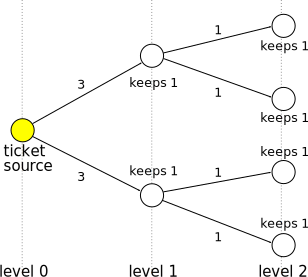
\includegraphics[width=0.9\linewidth]{sumup}
  \caption{Visualisation of the ticket distribution step of SumUp. Note that
    tickets are not distributed to nodes on the same level of breadth-first
    search, or nodes that already hold a ticket. The same process is also
    applied for GateKeeper, discussed in at the end of
    \autoref{sec:random-walk}.}
  \label{fig:sumup}
\end{figure}

Conversely, maximum flow is dual to minimum cut, so the problem of finding Sybil
can also be formulated as finding sparse cuts. The sparse cut problem is to find
a partition such that the ratio between the number in the cut and the number of
vertices in the smaller partition is minimised. Kurve and Kesidis devised an
algorithm for finding sparse cuts to detect sybils~\cite{kurve2011sybil}. It
relies on the presence of trusted nodes.

\subsection{Random Walk and OSN}\label{sec:random-walk}
Another family, possibly the largest, Sybil defence mechanism is based on random
walks in OSN (online social network), first proposed in
SybilGuard\cite{yu2006sybilguard}. The key assumptions in these techniques is
that the honest region is \emph{fast mixing}\footnote{In a graph, if a random
  walk of length $O(\log{N})$ reaches a stationary distribution of nodes, then
  the graph is fast mixing.}, and the attack edges are difficult to form and are
independent of the number of Sybils.

% The first
% defence mechanism is SybilGuard\cite{yu2006sybilguard}, created by Yu et el.
% SybilLimit\cite{yu2008sybillimit} is the continuation of SybilGuard and it is an
% improvement on many fronts while keeping the same or better guarantees as
% SybilGuard. In this section we focus on SybilLimit plus other random walk based
% techniques.

Before explaining the techniques, we define the terms \emph{random walk} and
\emph{random route} in the context of social graphs. In random walk, the social
graph is traversed such that outgoing edges are selected uniformly at random on
every hop of the walk. Random route is a modified form of a random walk. Every
node maintains a static routing table that contains a uniformly random
one-to-one mapping between incoming edges and outgoing edges, initialised at
start-up. Thus a route is determined by the tables on every node. An important
property of random route is that if two routes enter the same edge, then they
will always exit at the same edge, so their route after exiting will be exactly
the same. In most cases, the number of hops for a random route should be just
right, so that the fast mixing property is achieved in the honest region, this
is known as the \emph{mixing time}.

In SybilGuard~\cite{yu2006sybilguard}, every node acts as a verifier and
performs a single random route of a fixed length, determined by the mixing time.
The verifier treats every other nodes as suspects initially. The suspect is
labeled as an honest node if its random route intersects with the verificer's
random route. The number of accepted nodes for every intersection is limited by
a quota. The process is visualsed in \autoref{fig:sybilguard}. Intuitively, the
random route from an honest node is unlikely to escape into the Sybil region
because the number of attack edges is limited. The number of overlapping random
routes from the Sybils is bounded by the number of attack edges due to the
random route property. Recall that the number of attack edges is independent of
the number of Sybils, thus they are unlikely to intersect with many honest
nodes.

\begin{figure}
  \centering
  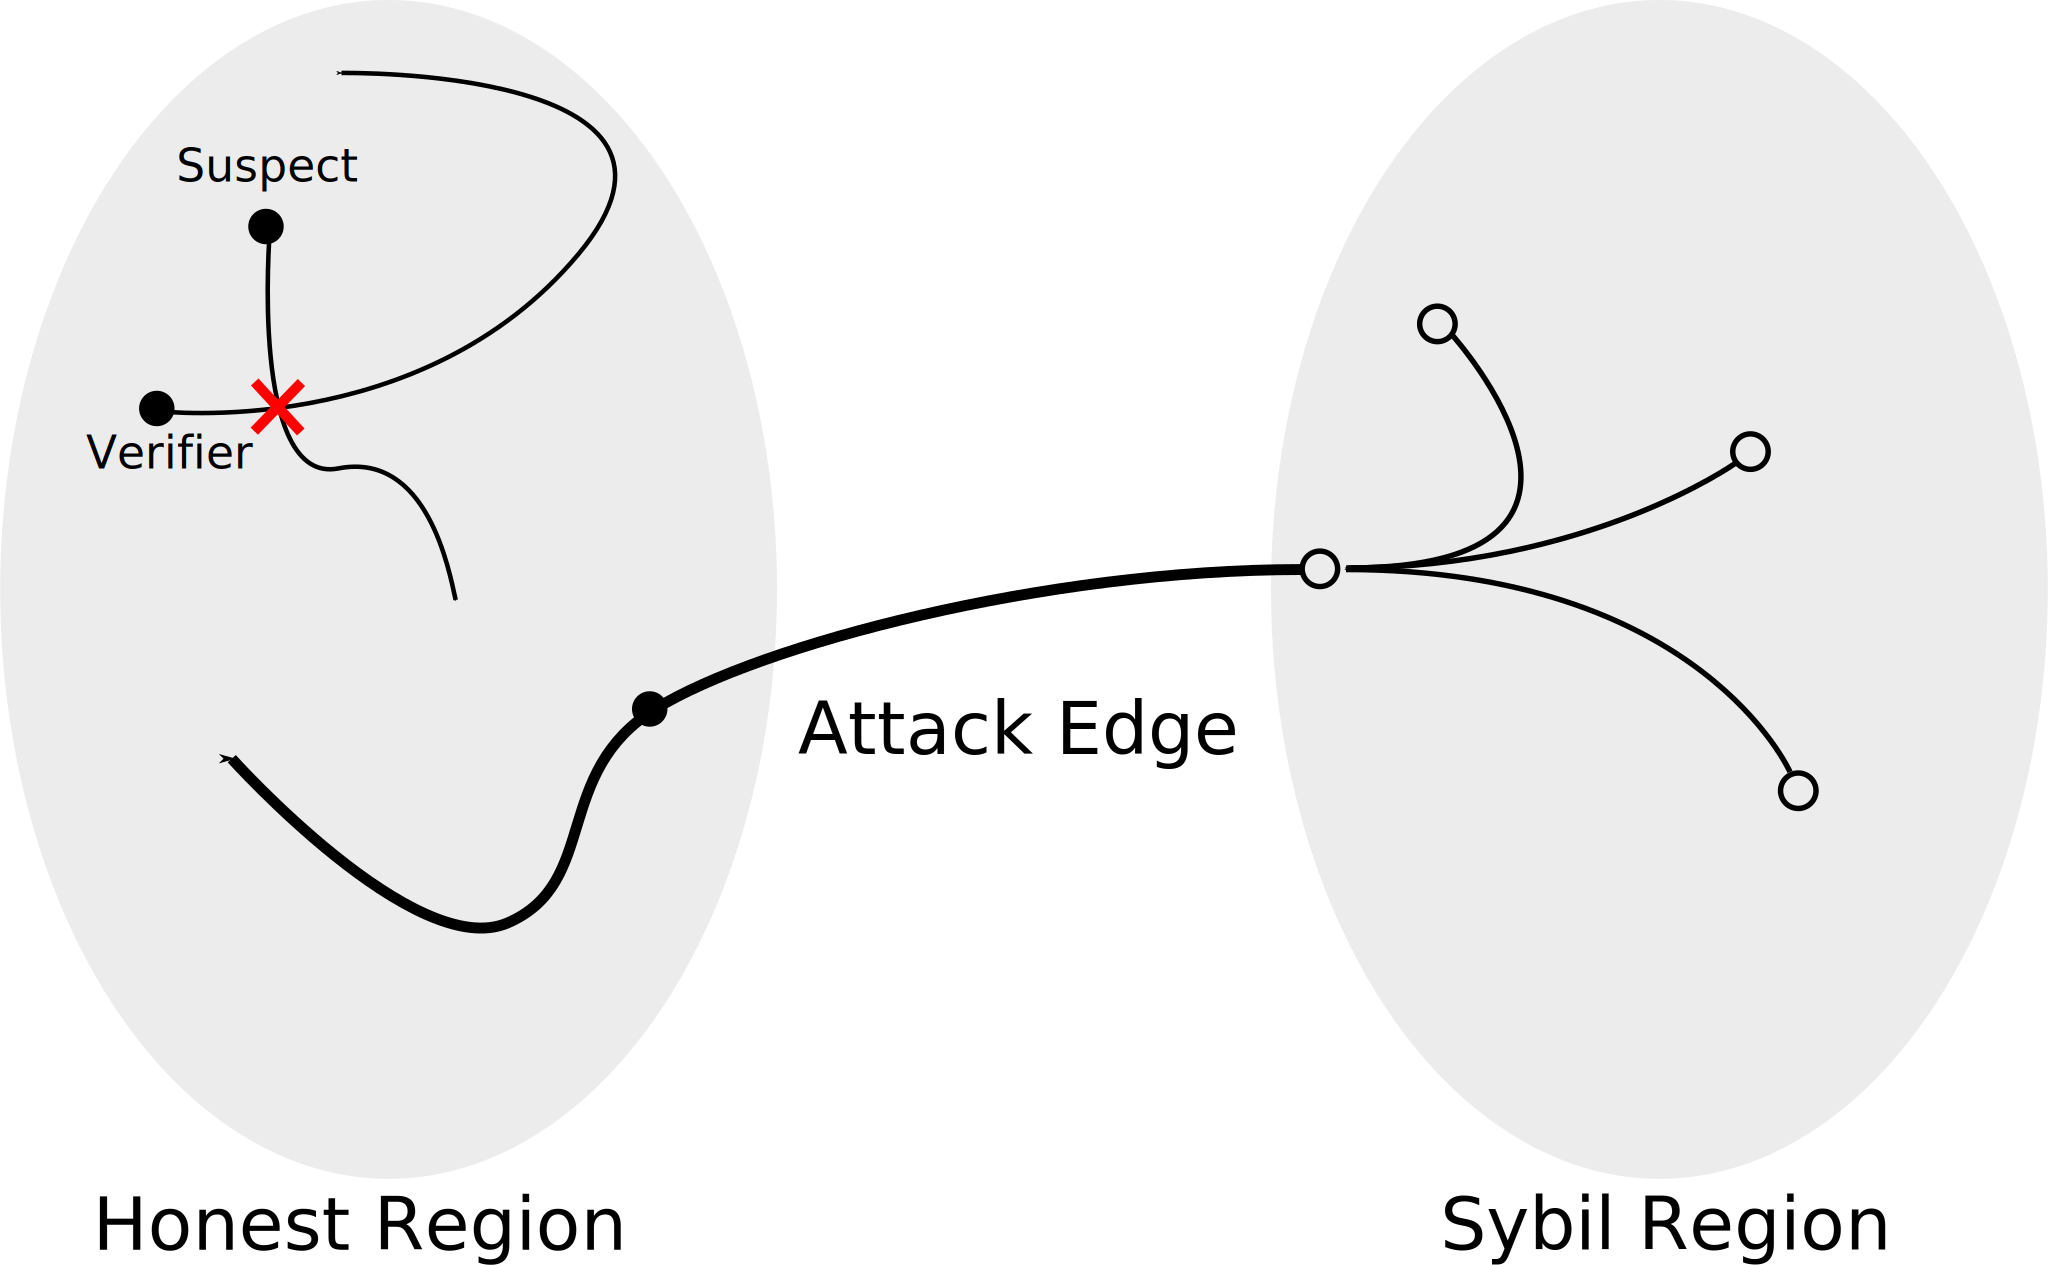
\includegraphics[width=\linewidth]{sybilguard}
  \caption{Visualisation of SybilGuard. The verifier accepts the suspect because
    their random routes intersect. The Sybils' random routes all come from a
    single attack edges, thus their routes are equivalent after entering the
    honest region.}
  \label{fig:sybilguard}
\end{figure}

SybilLimit~\cite{yu2008sybillimit} is the continuation of SybilGuard and it is
an improvement on many fronts while keeping the same or better guarantees. Same
as before, every honest node acts as a verifier $V$ and initially treats all
other nodes as suspects $S$. The verification process begins by performing
multiple independent random routes instead of a single one as in SybilGuard. $V$
labels $S$ as an honest node if and only if they share at least one tail (the
final edge in the route). For each tail of $V$, there is a quota for the number
of node that it labels. The authors prove that SybilLimit bounds the number of
accepted Sybils (false positives) at $O(\log{n})$, an improvement from
$O(\sqrt{n} \log{n})$ of SybilGuard. The process is visualised in
\autoref{fig:sybillimit}.

Let us consider the following three scenarios to intuitively show why SybilLimit
works. The same intuition applies to SybilGuard. Suppose $S$ is not a Sybil, and
if $V$ and $S$ perform enough random routes, each with enough hops for fast
mixing, then due to the Birthday Paradox, $S$ and $V$ will have an intersecting
tail with high probability. Next, suppose some of the tails of $V$ are in the
Sybil region so they may intersect with a large number of Sybils, but crossing
the attack edges is improbable and accepting a lot of Sybils is also difficult
due to the aforementioned quota mechanism, thus $V$ has a small probability of
accepting a large number of Sybils. Finally, consider there is only one attack
edge and suppose a Sybil has tails in the honest region, due to the random route
property, the route of the Sybils in the honest region will be equivalent
(overlapping), so accepting the Sybils in this scenario is also low due to the
quota mechanism.

\begin{figure}
  \centering
  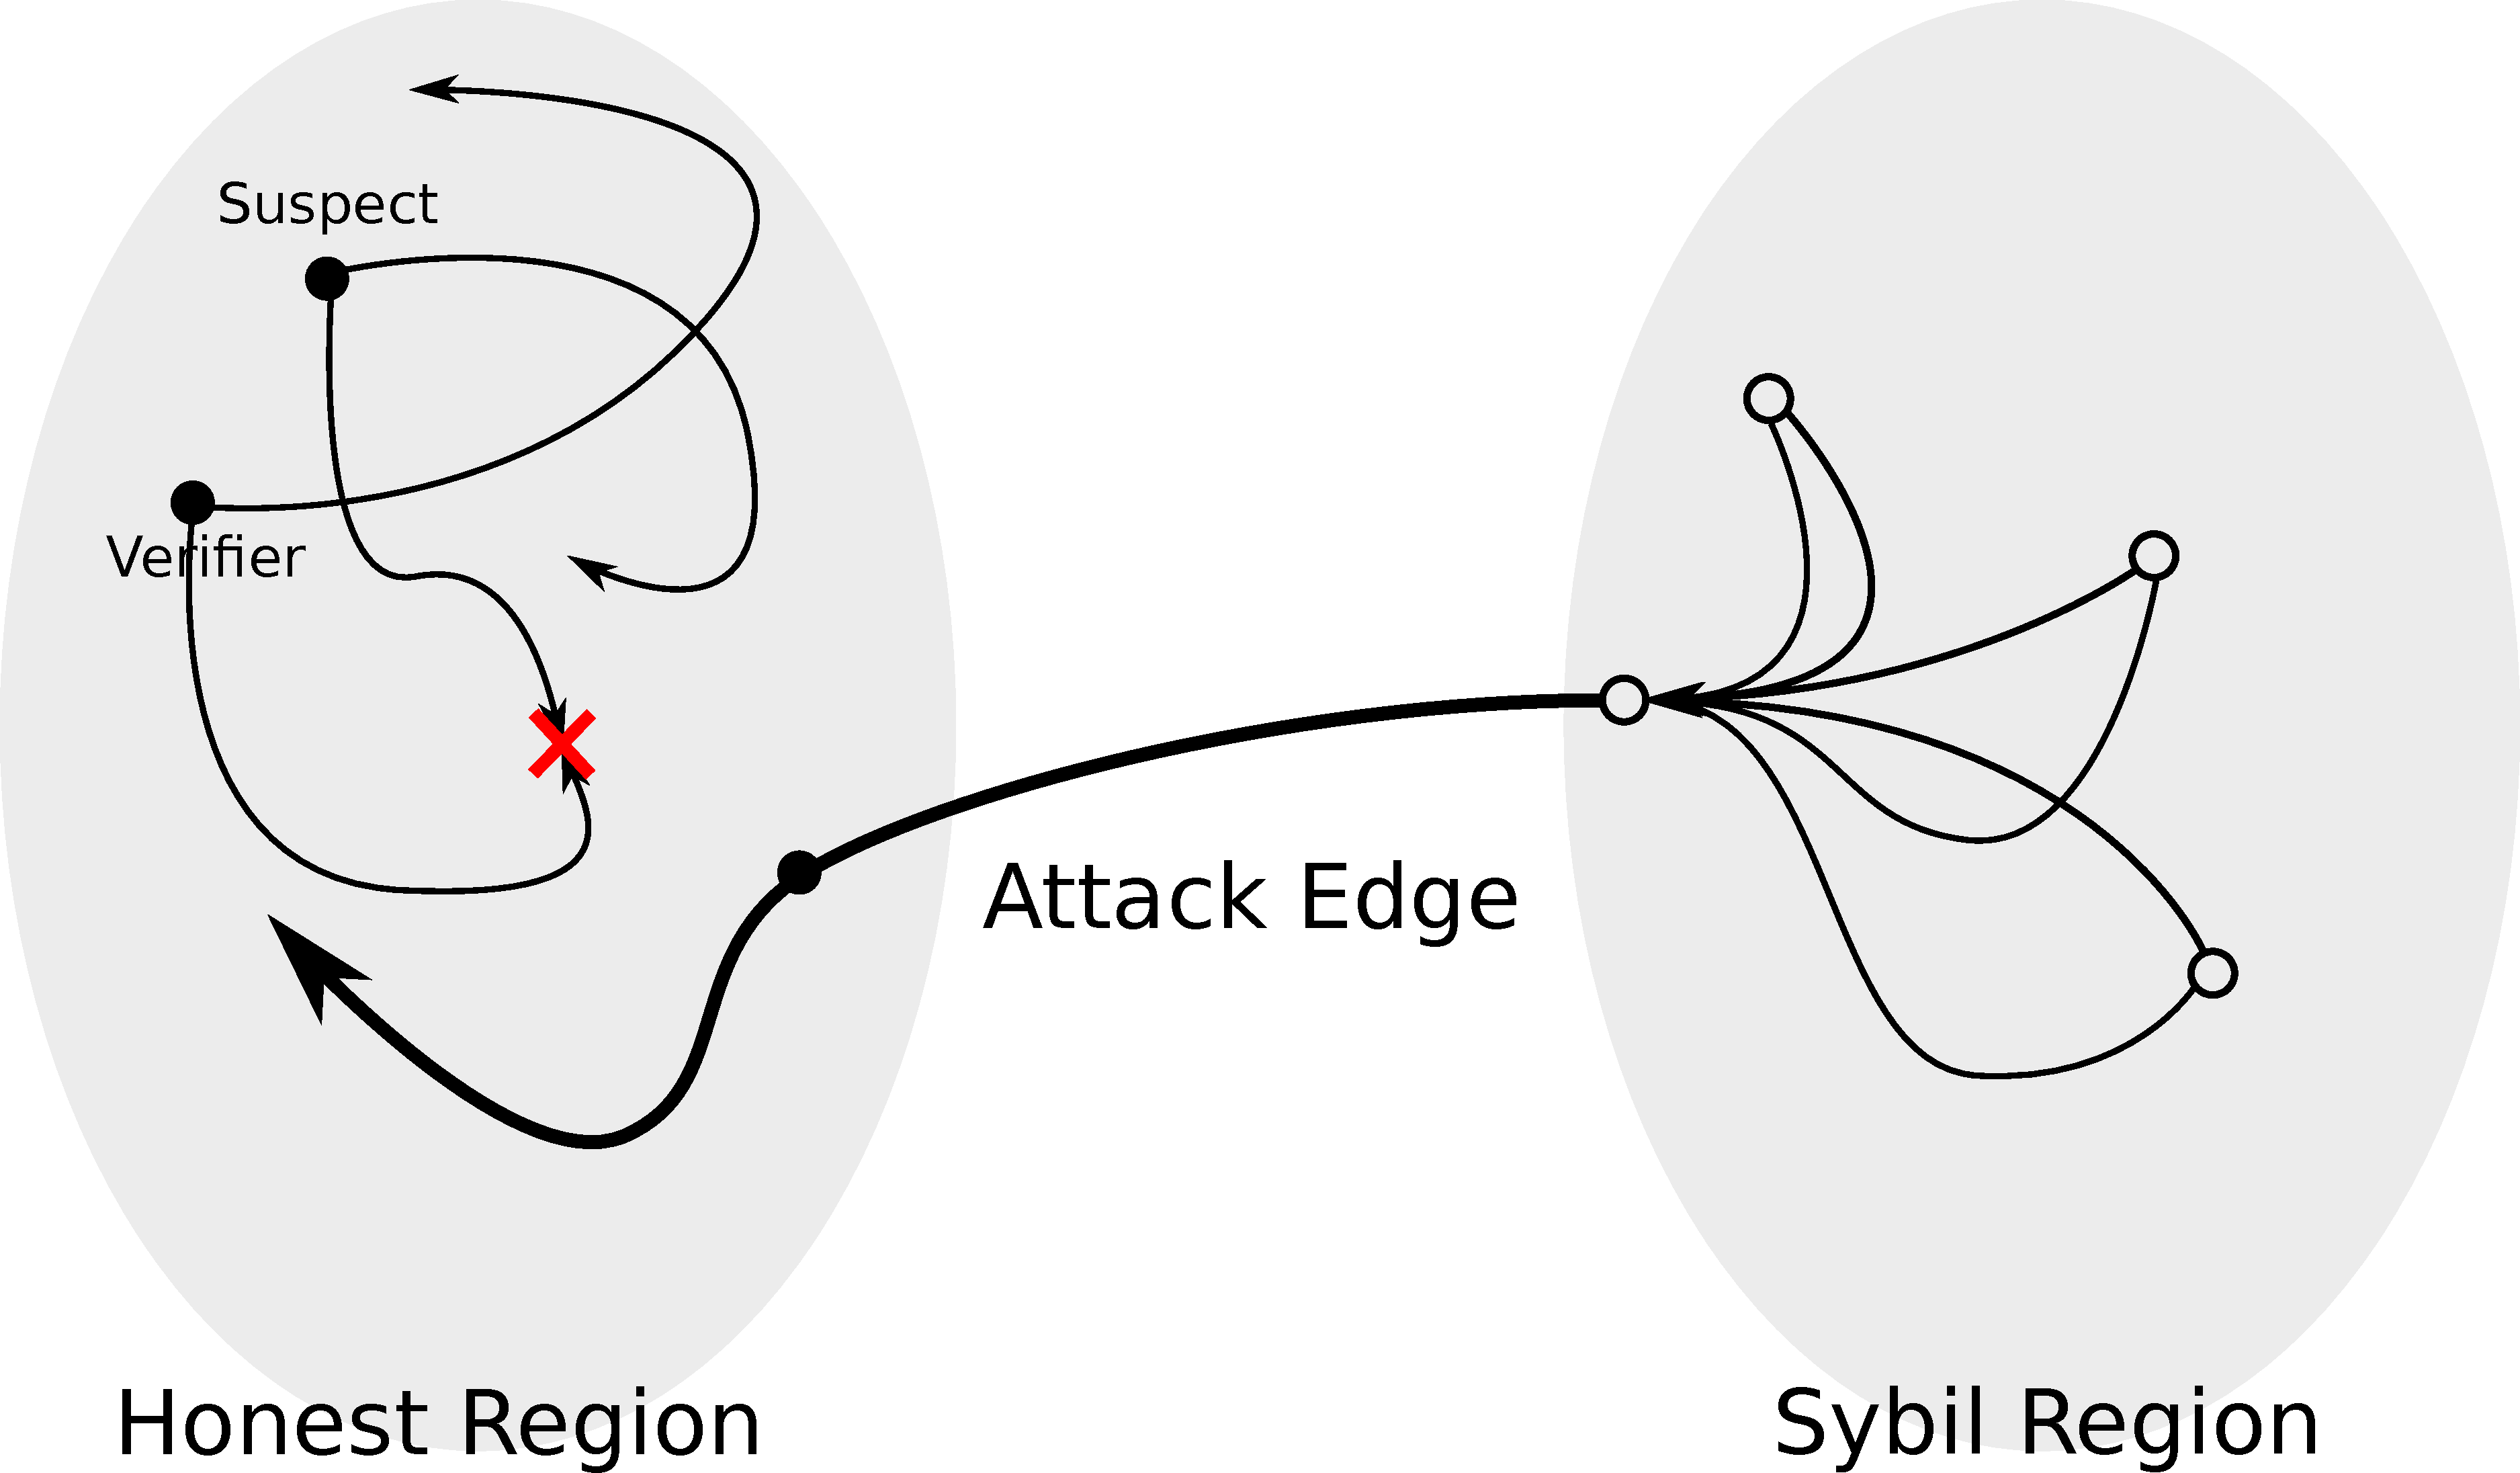
\includegraphics[width=\linewidth]{sybillimit}
  \caption{Visualisation of SybilLimit. The verifier accepts the suspect because
    one of the tails of their random routes meet. Similarly, the Sybils' random
    route are all from a single attack edges, so their routes are equivalent in
    the honest region.}
  \label{fig:sybillimit}
\end{figure}

SybilGuard and SybilLimit inspired many other defence mechanisms.
SybilInfer\cite{danezis2009sybilinfer} assumes trusted nodes, which create
traces by doing random walks in the graph. Based on the traces, a probability
model that descries the likelihood a trace $T$ was generated by a specific set
of honest nodes $X$, i.e. $\Pr[ T | X = \text{honest}]$. Then using Bayesian
inference, $\Pr[ X = \text{honest}| T ]$ can be computed, that is effectively
assigning a ``score'' to every node. Sybil are the nodes with a low ``score''.
SybilInfer outperforms SybilLimit regarding the number of false positives, but
its drawbacks are its high computational cost and reliance on trusted nodes.

Lesniewski et el. created Wh\={a}nau, a Sybil-resistent DHT, it is also inspired
by SybilLimit\cite{lesniewski2008sybil, lesniewski2010whanau}. Suppose all nodes
in the DHT belong to a social network and a node, say Alice (who is honest),
wish to join the DHT. Alice performs multiple random walks and it inserts the
node on the tails of her random walks into her own routing table. Again, the
random walk properties guarantee that there cannot be a large proportion of
Sybils in the routing table with a high probability. The number of entries in
the routing table needs to be high enough such that the entries cover the whole
key spaces. If Alice wants to find a key, she broadcasts the request to all the
entries. Since most of the entries are honest, Alice can retrieve the required
value with high probability.

SybilDefender~\cite{wei2012sybildefender} can be seen as a two step process. It
assumes the size of the Sybil region is smaller than the honest region and the
nodes in the Sybil region are well connected. The first step is to perform
random walk to detect Sybils. The second step is to detect a complete Sybil
region around the detected Sybils. The algorithm in the second step employs
\emph{partial} random walk, where the random walk is not allowed to traverse the
same node more than once. A property of partial random walks is that they
are likely to ``die'' (all the neighbour nodes have already been traversed) upon
reaching the edge of the Sybil region, thus they are likely to stay in the Sybil
region. The Sybil region is detected by examining the nodes traversed by the
partial random walk.

% how does SybilDefender guarantee that the Sybils actually perform the random
% walk correctly in the second step?

SybilRank~\cite{cao2012aiding}, in contrast of the aforementioned techniques, is
designed to be integrated with real-world OSN and is deployed on Tuenti (an OSN
with 11 million users). SybilRank uses short random walks that begins on trusted
nodes in the honest region. The trusted nodes is choosen manually, this allows
SybilRank to adapt to different graph structures. A novelty in SybilRank is that
it uses power iterations, an efficient technique for computing the landing
probability of random walks. Intuitively, the landing probability decreases for
nodes that are far away from the trusted nodes (since it is using short random
walks), especially for nodes in the Sybil region. The probabilities are
normalised by the degree of the node and then ranked. The potential Sybils are
the nodes that are under some threshold---a system parameter. Finally, various
actions can be performed to to verify the potential Sybils, e.g. using CAPTCHA
puzzles.

SybilShield~\cite{shi2013sybilshield} makes use of multiple communities
(\autoref{fig:community}). It begins the same way as
SybilGuard/SybilLimit, i.e. $V$ performs random route to determine whether
suspect $S$ is a Sybil. But to reduce the possibility that $S$ is in fact an
honest node but labeled as a Sybil, $V$ searches for agents $A$ that are from
another community. This is also done using random routes and relies on the
assumption that inter-community edges are rare. To do this, $V$ performs a
random route and picks a \emph{candidate} $A$, then $V$ and the candidate
perform random routes simultaneously, if they do not intersect then $A$ is
considered to be in another community, otherwise $V$ repeats the process until
it finds a suitable $A$. When a number of suitable $A$ is found, they all
perform random route and decides whether $S$ is actually a Sybil and then relay
the information back to $V$. If a large majority of $A$ say $S$ is honest, then
$V$ knows that it has made a mistake, otherwise $S$ is indeed a Sybil.
% the Algorithm 2 is not a community detection algorithm

\begin{figure}
  \centering
  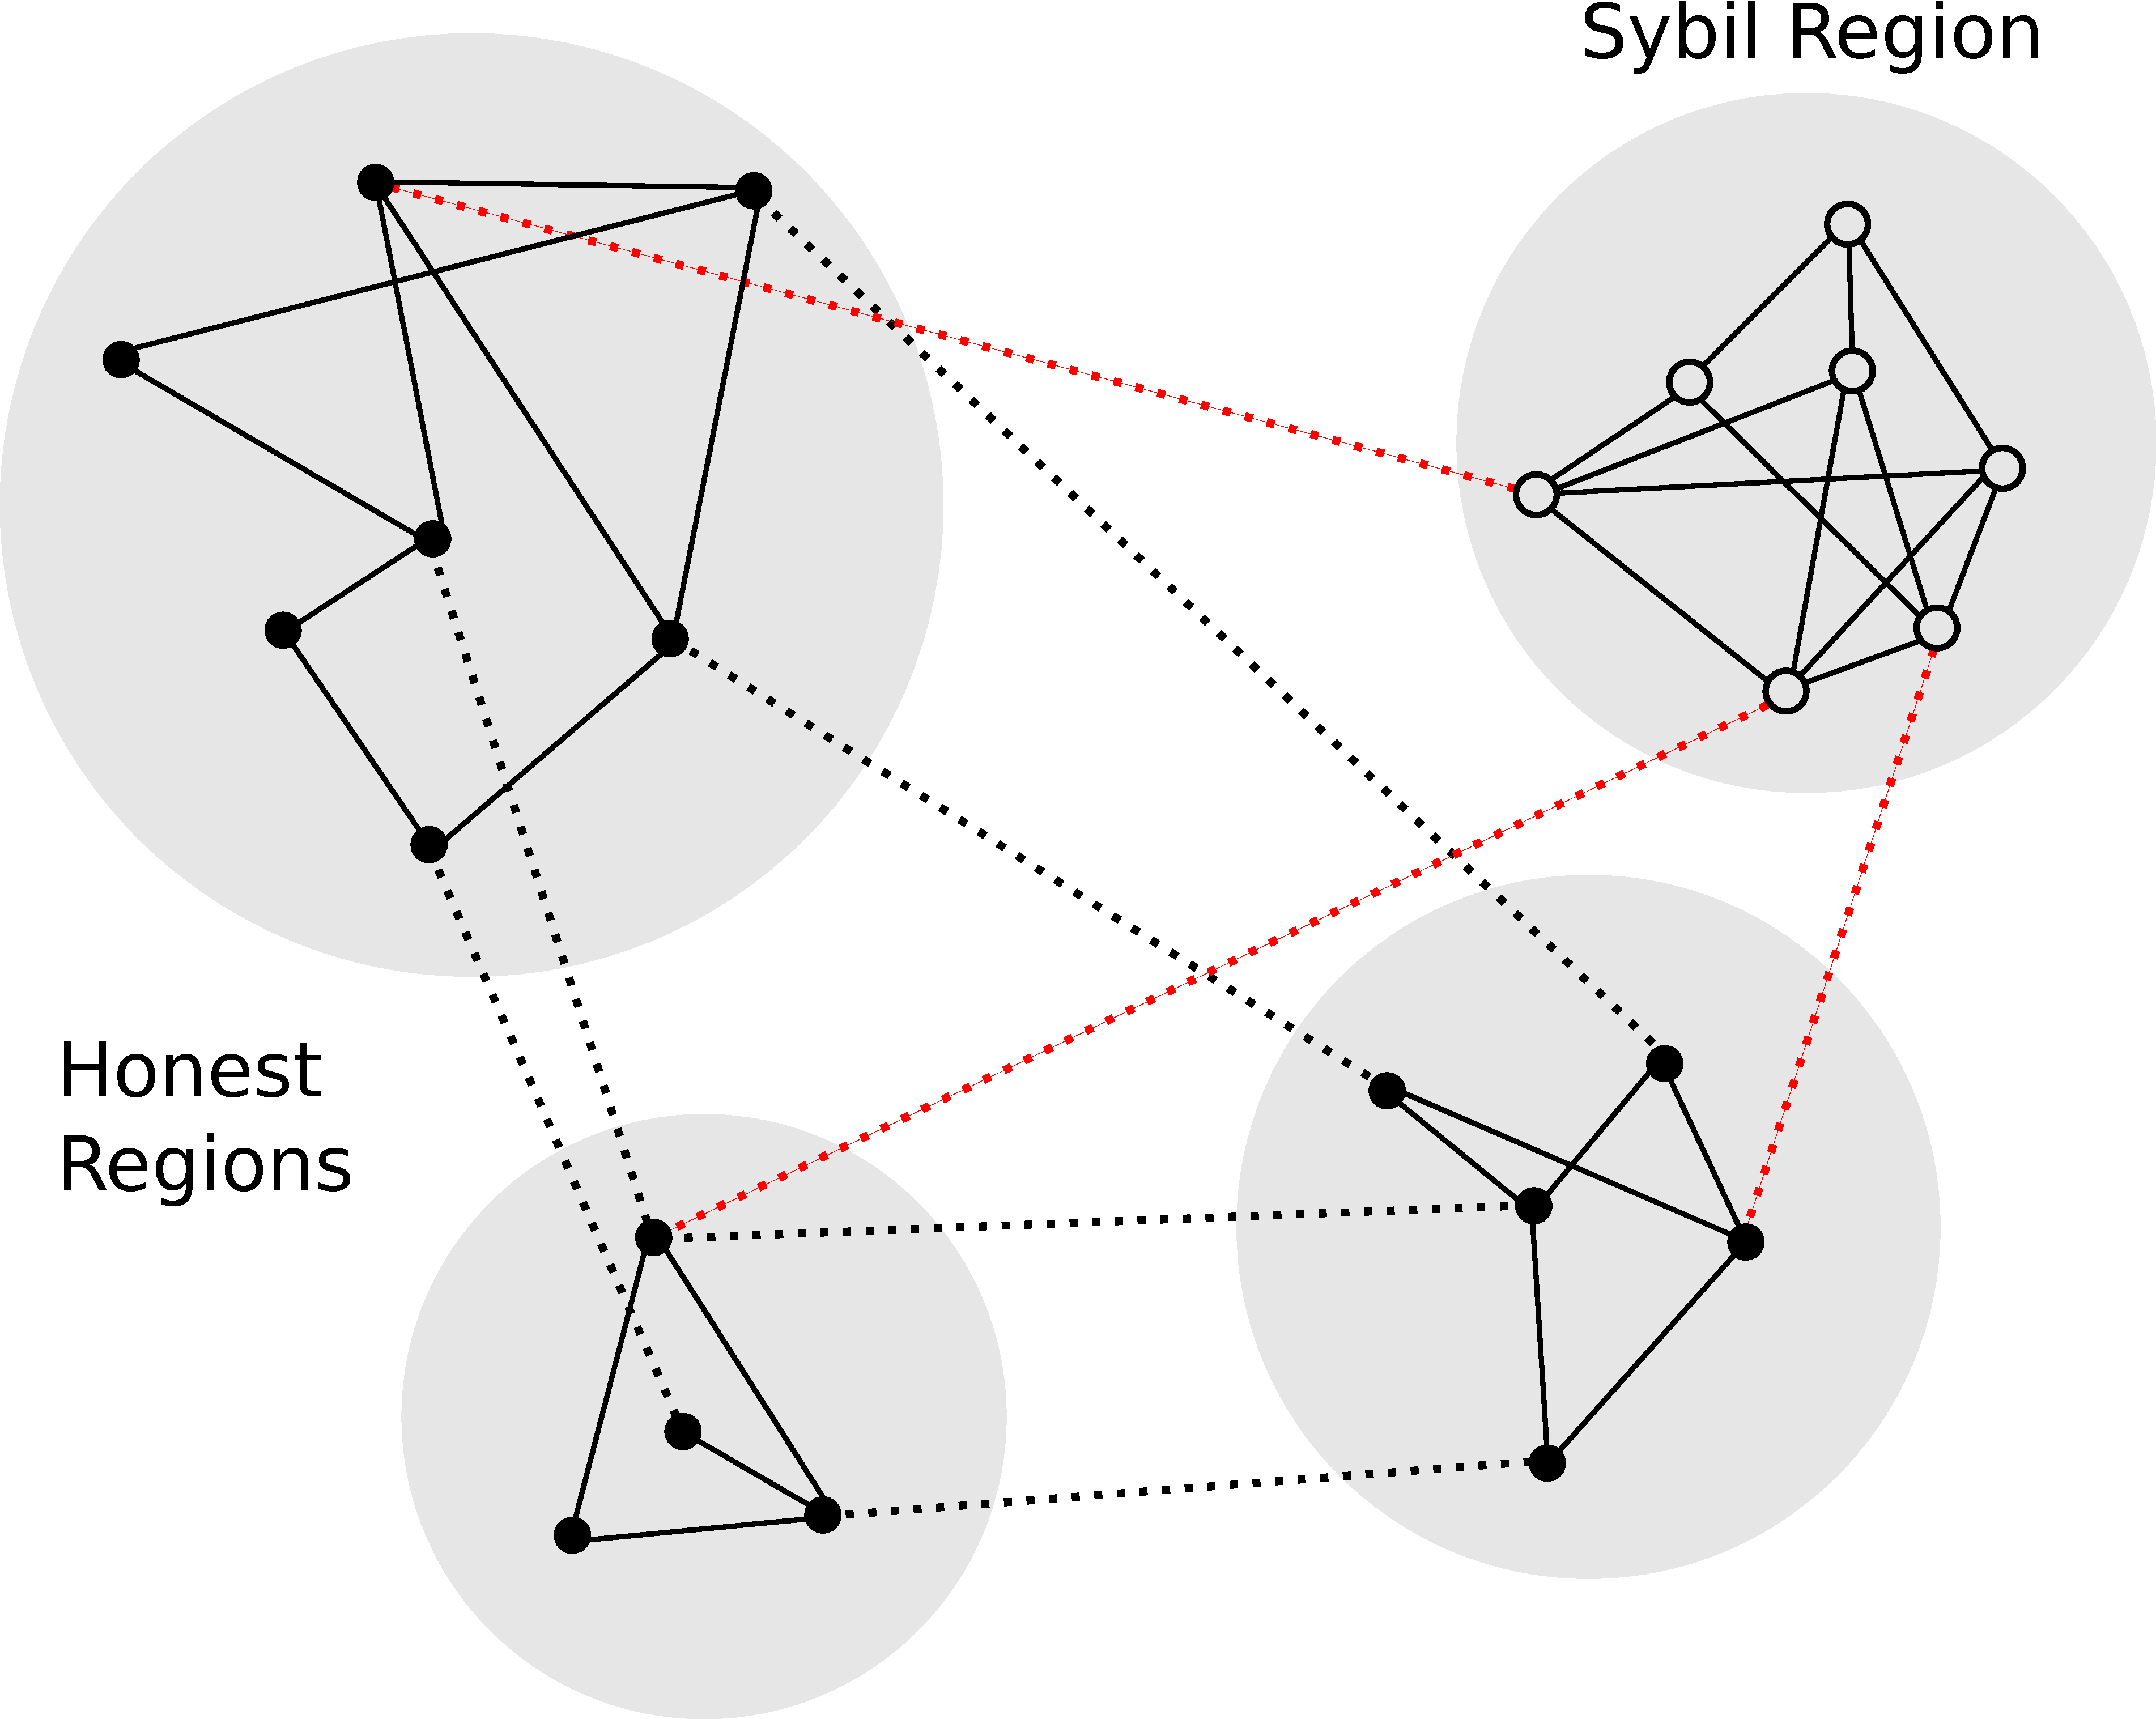
\includegraphics[width=0.9\linewidth]{community}
  \caption{Visualisation of communities in a social graph. Solid lines represent
    intra-community edges. Dotted lines represent inter-community edges. The red
    dotted lines are inter-community edges coming from the Sybils, in other
    words the attack edges. The idea of making use of communities is used in
    SybilShield as well as SybilExposer
    (\autoref{sec:community-detection}).}
  \label{fig:community}
\end{figure}

All the techniques so far use fixed length random walks. Recently, Liu et el.
argue that fixed length random walks is not adaquate because social graphs can
have communities of different sizes, nodes in a large community that is well
connected may have a lower mixing time than nodes in a smaller community. A
longer than desired random walk length will result in a growing number of false
negatives. To solve this problem, the authors created
SmartWalk\cite{liu2016smartwalk} which uses adaptive random walks. There are two
steps to SmartWalk. The first step uses machine learning to predict the local
mixing time given a node. The second step performs the random walk using the
local mixing time as the starting length, but on every hop the number of hops
remaining is also updated depending on the intermediate node's local mixing
time. Finally the Sybils can be detected using the same method as SybilLimit,
i.e. node is accepted when their tails meet. The authors evaluated SmartWalk
using real-world social graphs. In particular, the false positive rate for a
Twitter social graph can be reduced by two orders of magnitude when compared to
the standard SybilLimit.

GateKeeper~\cite{tran2011optimal} combines ideas from SumUp (discussed in
\autoref{sec:network-flow}) and SybilLimit. GateKeeper assumes a admission
controller that is honest, the admission controller performs random walks to
select $n$ ticket sources. The ticket sources act the same way as SumUp where it
distributes ticket in a breadth-first search manner (\autoref{fig:sumup}). For a
node to be labeled honest, it must obtain $fn$ tickets, where $f$ is a system
parameter (0.2 is shown to be a good value experimentally). This idea works
becauses if the ticket sources are evenly distributed and Sybils ony have a few
attack edges, then it is unlikely that they will receive a large number of
tickets.

% ReDS\cite{akavipat2014reds} suggests to use sybilimit or sybilinfer

\subsection{Community Detection}\label{sec:community-detection}
In this section we discuss techniques that leverage existing community detection
algorithm. The work started with Viswanath et al., who realised many of the
mechanisms mentioned in \autoref{sec:random-walk} such as SybilGuard, SybilLimit
and SybilInfer, are in fact performing local community detection (i.e. detecting
clusters of nodes) which is a more developed field~\cite{viswanath2010analysis}.
The authors also argue that social graphs are not always fast mixing, which may
result in poor results for techniques that use the fast mixing assumption.
Using synthetic social graphs, the authors show that applying Mislove's
algorithm~\cite{mislove2010you} achieve similar results as SybilLimit and
SybilInfer. But using a Facebook social graph, Mislove's algorithm performs
better.

The authors of SybilExposer~\cite{misra2016sybilexposer} argue that the number
of attack edges may not be that small which may render the random walk based
method ineffective. They proposed a solution that relies on the ratio between
the number of inter-community (inter-cluster) edges and the number of
intra-community (intra-cluster) edges. This is visualised in
\autoref{fig:community} where the sybil region has fewer
inter-community edges than the honest region. The idea is that this ratio is
different between honest communities and Sybil communities, namely the Sybil
communities have a lower ratio because they are well connected between
themselves but not with other honest communities. SybilExposer operates in two
stages, first communities are extracted using community detection algorithm (a
modified version of the Louvain method~\cite{blondel2008fast}), then the
communities are ranked based on the ratio and communities with a low ratio are
likely to be Sybils.
% community diversity vs node diversity

% SybilRadar\cite{mulamba2016sybilradar}

\subsection{Content Based and Machine Learning}
\label{sec:content-based}
In some application domains such as OSN it is possible to leverage user content
or user feedback to detect Sybils. These techniques work well in practice. But
often depend on uninformed attackers that do not try to mimic the behaviour of
honest nodes.

Ostra~\cite{mislove2008ostra} is a system for limit spam in social networks.
In the simplest form, every undirected edge in the social graph is considered as
two directed edges, each of them has a credit values. When a user wants to send
a message, it needs to find a path with enough credits in the social graph from
itself to the receiver. The edge traversed by the message will have its credit
deducted, and the opposite edge will have its credit added. The receiver then
decides whether the message is a spam, if it's not a spam then the credit
operations are reversed. Effectively, only spam messages will have an effect on
the credits. If a path cannot be found, i.e. all possible paths have run out of
credit, then the message is blocked. Naturally, spams from the Sybils must use
the attack edges, if enough honest users mark those messages as spam then the
credit on the attack edges will run out and the Sybils can no longer send
messages.

Stringhini et el. devised a machine learning technique to classify bot accounts
in Twitter~\cite{stringhini2010detecting}. User feedback is incoperated into the
features. For example one of features is ``FF Ratio'', that is the ratio between
number of users that the account is following and the number of followers. Other
features include ``URL Ratio'', ``Message Similarity'' and so on. The authors
collected data on ``honey-profiles'', trained a classifier after analysing those
data and collaborated with Twitter to delete tens of thousands of spam accounts.

VoteTrust~\cite{xue2013votetrust} leverages the distrust relationship, i.e.
friend request rejection, to detect Sybils in OSN. Suppose $A$ sends a friend
request to $B$, if $B$ accepts/rejects the request then it is considered as a
positive/negative vote on $A$ by $B$. The first step is to use PageRank combined
with human scrutiny to select a number of trust seeds in the honest region. Then
the trusted seeds distributes \emph{vote capacity}, that is the number of votes
each node can cast. Initially only the trusted seeds have a positive vote
capacity and other nodes have 0. When a node receives a positive vote from a
trusted seed, it also receives some vote capacity. Then it can repeat the same
process on nodes it votes on, thus distributing the vote capacity. The vote
capacity decreases as it goes further away from the trusted seeds. This
technique is comparable to the ticket distribution technique used in SumUp and
GateKeeper. Finally, the votes are aggregated to compute a global ration for
every node in the graph. Naturally, the Sybils are likely to have a low vote
because their vote capacity is low and many of their friend requests would be
rejected.

Integro\cite{boshmaf2015integro} is a hybrid between random walk and content
based approaches. It begin by training a machine learning algorithm to identify
potential \emph{victim accounts}, that is honest accounts that have accepted
Sybils as their friends. Then in the social graph, edges connecting the
potential victim accounts will have its weight reduced depending on the
likelihood of it being a victim. Finally, perform biased short random walk
starting from some known honest account to compute the landing probabilities for
every node. Biased in a sense that that the walk is a higher probability of
using a path with a higher weight. Sybils are the nodes with a low landing
probabilty. This technique works because, victims are easier to detect than
Sybils due to the fact that Sybils can arbitrarily modify their account
information to avoid detection. Once the victims are detected, they effectively
form a ``border-line'' between the honest region and the Sybil region. Finally,
it is unlikely that the random walk will traverse into the Sybil region due to
its bias, so the Sybil will have a low landing probability and be detected.

% \subsection{Content Driven}
% \cite{chatterjee2008robust}

\subsection{Other}
There are many defence mechanisms that unique in their own right. We cover some
of them in this section.

Trust transfer\cite{seigneur2005trust} is a Sybil defence mechanism for
reputation systems that transfers the reputation score from a recommender to a
recommended identity. This method discourages self-recommendation behaviour
because the attacker would need to lower the reputation of its Sybils to
recommend him or herself. The Sybils cannot gain reputation from honest
identities because if they do not interact with them. It may be strange to lose
reputation when recommending an identity, but the authors argue that in certain
scenarios where there are a lot of interactions and the overall trustworthieness
is high, then there is no major effect to transfer a little bit of reputation to
a recommended identity.

Yu et el. of DSybil\cite{yu2009dsybil} argue that defending Sybils in reputation
or recommendation systems is a lot more difficult than in social networks
because only a very small percentage of the user will vote for an object (e.g.
news article in Reddit), so a small number of Sybils and attack edges can easily
out-vote honest users. Their proposed solution is DSybil, a distributed
algorithm for diminishing the influence of Sybils in recommendation systems
using historical data. Suppose Alice is an identity that runs the algorithm, and
every identity begins with the same trust score from Alice's perspective. The
algorithm runs in rounds. In every round, Alice picks an object to consume (e.g.
reads the new article on Reddit) and then makes a binary (good or bad) feedback
on the object. Then Alice computes whether the object is \emph{overwhelming},
namely whether the sum of the trust scores of the voters of the object exceeds
some threshold. If Alice voted for good and the object is not overwhelming, then
she would increase the trust scores by some factor for all the voters of that
object. Otherwise she decreases the trust score by some factor. When Alice needs
a recommendation, a uniformly random overwhelming object is returned. Trust
scores for identities that have the same interest as Alice grow exponentially
when Alice consumes a good non-overwhelming object. Conversely the trust scores
decreases exponentially for identities that are recommending bad objects, making
Sybils ineffective.
% Similar to some randomised byzantine agreement algorithm?

SyMon\cite{jyothi2009symon} or \emph{Sybil Monitor} assumes that any two
sufficiently random nodes in the network cannot both be Sybils with a high
probability. Then the nodes are paired together to monitor each other's
transactions. For instance, a transaction could be reporting the number bytes
transferred in a P2P file sharing network. Cheating occurs when a node reports
some bytes transferred that does not match its network traffic. The authors
provide four methods for pairing nodes. Suppose the nodes are identified by a
cryptographically secure hash of their RSA public key, then it is difficult to
create identities deterministically. Nodes can be matched by the closeness of
their identities. The downside of this approach is that it sacrifices a lot of
privacy, every action that a node makes is monitored by some other node.

% SybilFrame?

\begin{comment}
\subsection{Cryptography Based Techniques?}
Secure-Overlay\cite{lua2007securing} - ID crypto and SSS
Privacy-preserving\cite{schaub2016trustless} - blockchain?
Proof-of-stake\cite{dennis2016rep}

\subsection{Unsorted}

Beth and PGP limits Sybil attack to some extent by using social graphs
Beth 94\cite{beth1994valuation}
PGP (Zimmermann) 95\cite{zimmermann1995official}

Yu 00\cite{yu2000social}
% CORE 02\cite{michiardi2002core} % MANETs
Lee 03\cite{lee2003cooperative} - uses flooding, might not be scalable, only talks about DoS
% Buchegger 04 - MANETs
% Xiong 03\cite{xiong2003reputation} % also PeerTrust?
Marti 04\cite{marti2004limited}
ARA 05\cite{ham2005ara} - no mention of sybil, prevents freeriding, prevents short-term abuse because reputation increases gradually
FuzzyTrust Song 05\cite{song2005trusted} - uses fuzzy logic
P2PRep/Fuzzy 06\cite{aringhieri2006fuzzy} - also fuzzy, does not prevent generation of false rumors
Xiong 05\cite{xiong2007countering} - no mention of sybil, but tries to mitigate false information
PowerTrust 06\cite{zhou2007powertrust} - uses ``power nodes'' (from power-law), no mention of sybil, some defence against colluders
% Li 07 - MANETs

Histos and Sopras\cite{zacharia2000collaborative}, doesn't really have structure?
Beta\cite{jsang2002beta}
% Confidant\cite{buchegger2002performance} MANETs
Gupta et al.\cite{gupta2003reputation}

PeerTrust\cite{xiong2004peertrust} - DHT, used P-GRID source code, has credibility rating

PerContRep\cite{yan2014percontrep}


\subsection{Does not handle Sybil-attack}
TrustMe\cite{singh2003trustme} is a reputation that focuses on anonymity, no mention of sybil attack

H-Trust\cite{zhao2009htrust} does not mention sybil

Coner et al.\cite{conner2009trust} assumes clients cannot perform sybil attack

TrustGuard 05\cite{srivatsa2005trustguard} - assumes it is built on secure overlay networks (sybil-proof networks)

Scrivener 05\cite{nandi2005scrivener} - assumes ID cannot be created and discarded

\end{comment}
%%% Local Variables:
%%% mode: latex
%%% TeX-master: "main"
%%% End:
